\documentclass[a4paper,12pt]{article}
\usepackage[a4paper, margin=1in]{geometry} % Sets the paper size to A4 and margins to 1 inch
\usepackage{graphicx}
\usepackage{subcaption} % for subfigures
\usepackage{setspace}		
\usepackage{xcolor,listings} % for typesetting code
\usepackage{enumitem}
\usepackage{tabularx}


\lstset{
    upquote=true,
    language=SQL,
    showspaces=false,
    basicstyle=\ttfamily,
    keywordstyle=\bfseries\color{blue!60},
    numbers=left,
    numberstyle=\tiny,
    commentstyle=\color{gray},
    backgroundcolor=\color{gray!10}
}

\begin{document}
\begin{titlepage}
    
%% Adding logo
\begin{figure}[h]
		\vspace*{-1em}
		\centering
		
\includegraphics[width=0.2\linewidth]{university_logo.png}
		\par
		\vspace*{2em}
		{\Large UNIVERSITY OF CHITTAGONG}
\end{figure}
%% Document information
\begin{center}
		\vspace*{3em}
		\textbf{Department of Computer Science and Engineering} \\
		\bigskip
		Session: 2021-2022 \\
		4th semester \\
		\bigskip
		\begin{tabular}{l l}
		  Assignment No. &: 1\\
		  Course Title &: Database Systems \\
		  Course Code No. &: CSE-413 \\
		\end{tabular}
\end{center}

%% Teacher information
\begin{center}
		\vspace*{3em}
		Submitted to: \\
		\textbf{Dr. Rudra Pratap Deb Nath} \\
		Associate Professor \\
		Department of Computer Science and Engineering \\
		University of Chittagong
\end{center}

%% Student information
\begin{center}
		\vspace*{3em}
		Submitted by: \\
		\textbf{Sanzid Islam Mahi} \\
		ID: 22701065 \\
		Department of Computer Science and Engineering \\
		University of Chittagong
\end{center}




\begin{center}
	\vspace*{3em}
	Date: Jul 02, 2024
\end{center}
\end{titlepage}
%% Book Name %%
% \newpage
%%%%%%%%%%%%%%% Book Name %%%%%%%%%%%%%%%
\begin{center}
        \textbf{\LARGE Oracle9i SQL-I}
\end{center}

\section*{Chapter 9}
\subsection*{Practice 9}
\begin{enumerate}

%%%%%%%%% Problem 1 %%%%%%%%%%%
\item Create the DEPT table based on the following table instance chart. Place the
syntax in a script called \texttt{lab9\_1.sql}, then execute the statement in the script to create the table.
Confirm that the table is created
\begin{figure}[h]
\centering
    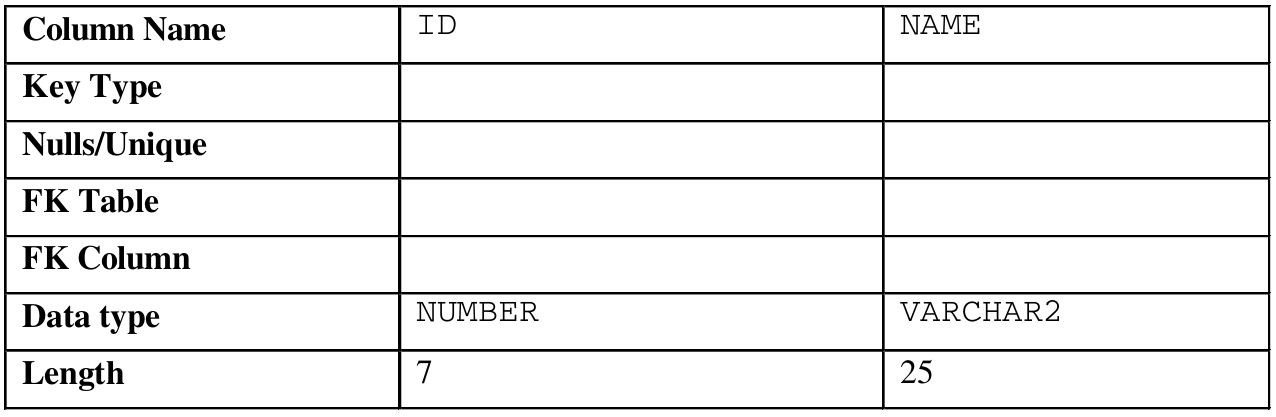
\includegraphics[width=.7\linewidth]{graphics/91.png}
\end{figure}

\textbf{Solution: }
\begin{lstlisting}[language=SQL]
CREATE TABLE dept(
    ID INT (7),
    NAME VARCHAR(25)
);

DESCRIBE DEPT;
\end{lstlisting}
\textbf{Output: }
\begin{figure}[h]
    \centering
    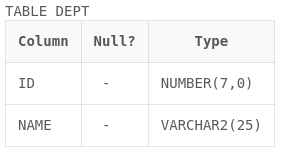
\includegraphics[width=0.5\linewidth]{graphics/p91.png}
\end{figure}

%%%%%%%%% Problem 2 %%%%%%%%%%%
\item Populate the DEPT table with data from the DEPARTMENTS table. Include only columns that
you need.

\textbf{Solution: }
\begin{lstlisting}[language=SQL]
INSERT INTO dept
SELECT department_id, department_name
FROM departments;
\end{lstlisting}

%%%%%%%%% Problem 3 %%%%%%%%%%%
\item Create the EMP table based on the following table instance chart. Place the syntax in a script called
\texttt{lab9\_3.sql}, and then execute the statement in the script to create the table. Confirm that the table is
created.
\begin{figure}[h]
\centering
    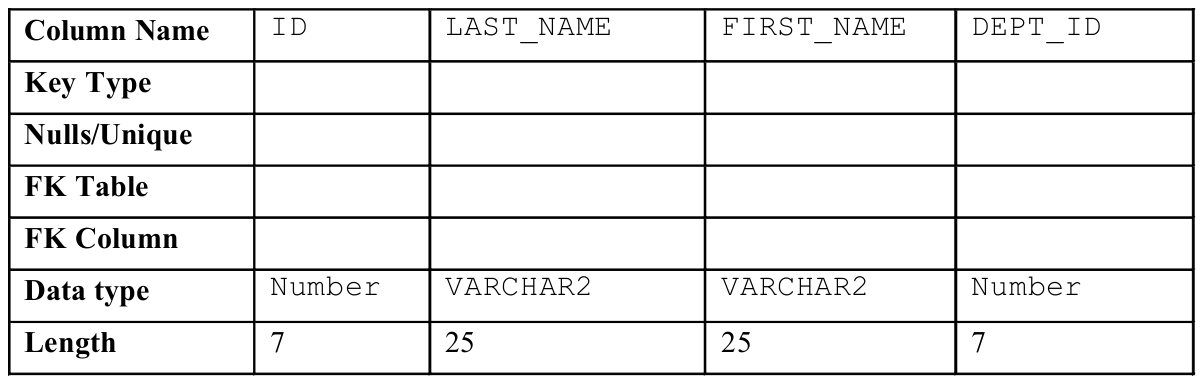
\includegraphics[width=.7\linewidth]{graphics/93.png}
\end{figure}

\textbf{Solution: }
\begin{lstlisting}[language=SQL]
CREATE TABLE emp(
    id int (7),
    last_name varchar(25),
    first_name varchar(25),
    dept_id int (7)
);

DESCRIBE emp;
\end{lstlisting}
\textbf{Output: }
\begin{figure}[h]
    \centering
    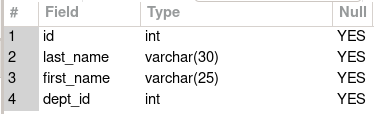
\includegraphics[width=0.5\linewidth]{graphics/p93.png}
\end{figure}

%%%%%%%%% Problem 4 %%%%%%%%%%%
\item Modify the EMP table to allow for longer employee last names. Confirm your modification.
\begin{figure}[h]
\centering
    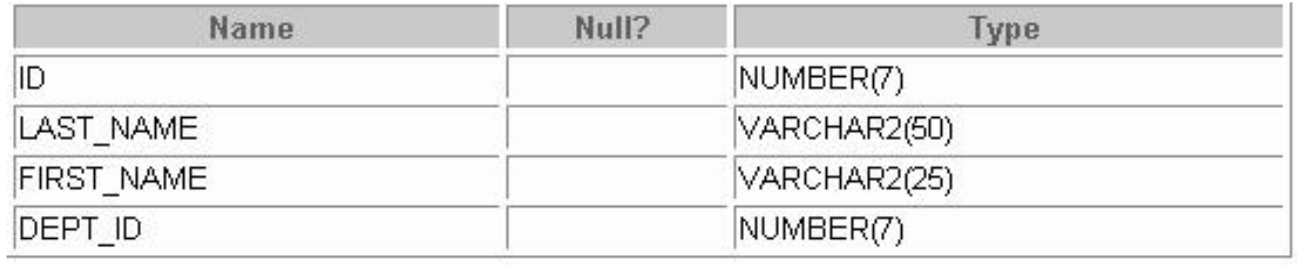
\includegraphics[width=.7\linewidth]{graphics/94.png}
\end{figure}

\textbf{Solution: }
\begin{lstlisting}[language=SQL]
ALTER TABLE emp
MODIFY last_name VARCHAR(50);

DESCRIBE emp;
\end{lstlisting}
\textbf{Output: }
\begin{figure}[h]
    \centering
    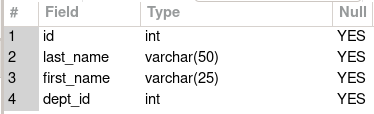
\includegraphics[width=0.5\linewidth]{graphics/p94.png}
\end{figure}

%%%%%%%%% Problem 5 %%%%%%%%%%%

\item Confirm that both the DEPT and EMP tables are stored in the data dictionary. (Hint:
\texttt{USER\_TABLES})
\begin{figure}[h]
\centering
    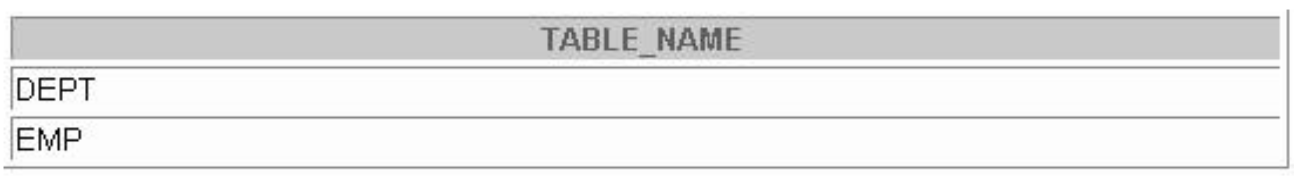
\includegraphics[width=.5\linewidth]{graphics/95.png}
\end{figure}

\textbf{Solution: }
\begin{lstlisting}[language=SQL]
SELECT table_name
FROM information_schema.tables
WHERE table_name IN ('dept', 'emp');
\end{lstlisting}
\textbf{Output: }
\begin{figure}[h]
    \centering
    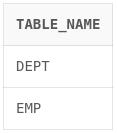
\includegraphics[width=0.5\linewidth]{graphics/p95.png}
\end{figure}

%%%%%%%%% Problem 6 %%%%%%%%%%%
\item Create the EMPLOYEES2 table based on the structure of the EMPLOYEES table. Include only the
EMPLOYEE\_ID, FIRST\_NAME, LAST\_NAME, SALARY, and DEPARTMENT\_ID columns. Name
the columns in your new table ID, FIRST\_NAME, LAST\_NAME, SALARY , and DEPT\_ID,
respectively.

\textbf{Solution: }
\begin{lstlisting}[language=SQL]
CREATE TABLE employees2 AS
SELECT employee_id id, first_name, last_name, salary,
    department_id dept_id
FROM employees;
\end{lstlisting}

%%%%%%%%% Problem 7 %%%%%%%%%%%
\item Drop the EMP table.

\textbf{Solution: }
\begin{lstlisting}[language=SQL]
DROP TABLE emp;
\end{lstlisting}

%%%%%%%%% Problem 8 %%%%%%%%%%%
\item Rename the EMPLOYEES2 table as EMP.

\textbf{Solution: }
\begin{lstlisting}[language=SQL]
RENAME TABLE employees2 TO emp;
\end{lstlisting}

%%%%%%%%% Problem 9 %%%%%%%%%%%
\item Add a comment to the DEPT and EMP table definitions describing the tables. Confirm your
additions in the data dictionary.

\textbf{Solution: }
\begin{lstlisting}[language=SQL]
ALTER TABLE dept
COMMENT = 'This table stores department information';

ALTER TABLE emp
COMMENT = 'This table stores employee information';

SELECT table_name, table_comment
FROM information_schema.tables
WHERE table_name IN ('dept', 'emp');
\end{lstlisting}
\textbf{Output: }
\begin{figure}[h]
    \centering
    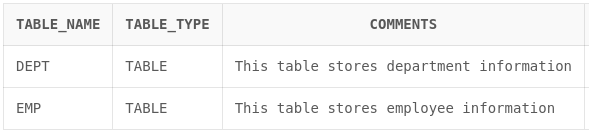
\includegraphics[width=0.8\linewidth]{graphics/p99.png}
\end{figure}

%%%%%%%%% Problem 10 %%%%%%%%%%%
\item Drop the \texttt{FIRST\_NAME} column from the EMP table. Confirm your modification by checking the
description of the table.

\textbf{Solution: }
\begin{lstlisting}[language=SQL]
ALTER TABLE emp
DROP COLUMN first_name;

DESCRIBE emp;
\end{lstlisting}
\textbf{Output: }
\begin{figure}[h]
    \centering
    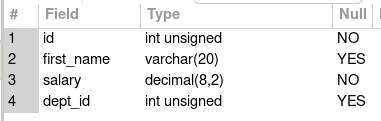
\includegraphics[width=0.5\linewidth]{graphics/p910.png}
\end{figure}

%%%%%%%%% Problem 11 %%%%%%%%%%%
\item In the EMP table, mark the \texttt{DEPT\_ID} column as UNUSED. Confirm your
modification by checking the description of the table.

\textbf{Solution: }
\begin{lstlisting}[language=SQL]
ALTER TABLE emp
SET UNUSED COLUMN dept_id;

DESCRIBE emp;
\end{lstlisting}
\item Drop all the UNUSED columns from the EMP table. Confirm your modification by checking the
description of the table.

\textbf{Solution: }
\begin{lstlisting}[language=SQL]

\end{lstlisting}
% \textbf{Output: }
% \begin{figure}[h]
%     \centering
%     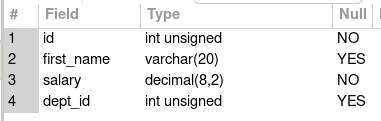
\includegraphics[width=0.5\linewidth]{graphics/p910.png}
% \end{figure}
\end{enumerate}


\newpage
\section*{Chapter 10}
\subsection*{Practice 10}
\begin{enumerate}

%%%%%%%%% Problem 1 %%%%%%%%%%%
\item Add a table-level PRIMARY KEY constraint to the EMP table on the ID column. The constraint
should be named at creation. Name the constraint \texttt{my\_emp\_id\_pk}.\\
\textbf{Hint: }The constraint is enabled as soon as the ALTER TABLE command executes
successfully.

\textbf{Solution: }
\begin{lstlisting}[language=SQL]
ALTER TABLE emp
ADD CONSTRAINT my_emp_id_pk PRIMARY KEY (id);
\end{lstlisting}
\textbf{Output: }
% \begin{figure}[h]
%     \centering
%     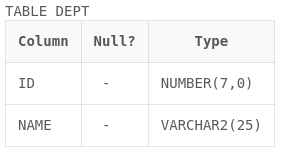
\includegraphics[width=0.5\linewidth]{graphics/p91.png}
% \end{figure}

%%%%%%%%% Problem 2 %%%%%%%%%%%
\item Create a PRIMARY KEY constraint to the DEPT table using the ID column. The constraint should
be named at creation. Name the constraint \texttt{my\_deptid\_pk}.\\
\textbf{Hint: }The constraint is enabled as soon as the ALTER TABLE command executes
successfully.

\textbf{Solution: }
\begin{lstlisting}[language=SQL]
ALTER TABLE dept
ADD CONSTRAINT my_deptid_pk PRIMARY KEY(id);
\end{lstlisting}

%%%%%%%%% Problem 3 %%%%%%%%%%%
\item Add a column \texttt{DEPT\_ID} to the EMP table. Add a foreign key reference on the EMP table that
ensures that the employee is not assigned to a nonexistent department. Name the constraint
\texttt{my\_emp\_dept\_id\_fk}.

\textbf{Solution: }
\begin{lstlisting}[language=SQL]
ALTER TABLE emp
ADD (dept_id NUMBER(7));
ALTER TABLE emp
ADD CONSTRAINT my_emp_dept_id_fk
FOREIGN KEY (dept_id) REFERENCES dept(id);
\end{lstlisting}
% \textbf{Output: }
% \begin{figure}[h]
%     \centering
%     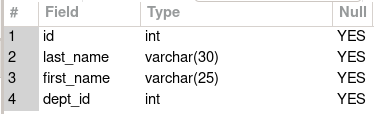
\includegraphics[width=0.5\linewidth]{graphics/p93.png}
% \end{figure}

%%%%%%%%% Problem 4 %%%%%%%%%%%
\item Confirm that the constraints were added by querying the \texttt{USER\_CONSTRAINTS} view. Note the
types and names of the constraints. Save your statement text in a file called \texttt{lab10\_4.sql}.
\begin{figure}[h]
\centering
    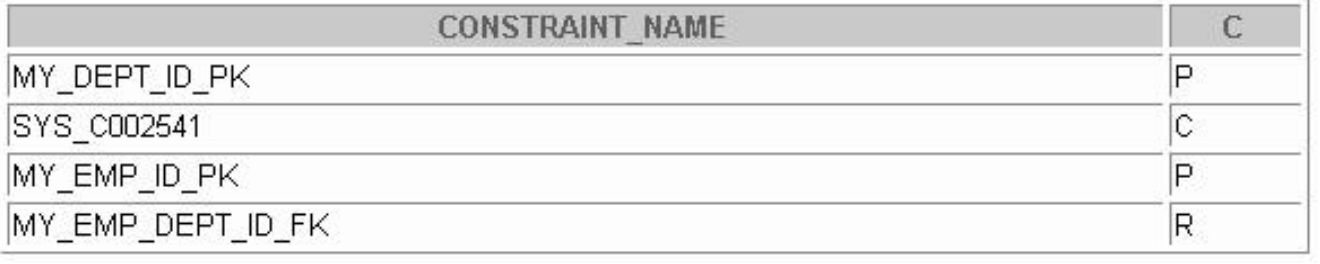
\includegraphics[width=.8\linewidth]{graphics/104.png}
\end{figure}

\textbf{Solution: }
\begin{lstlisting}[language=SQL]
select constraint_name, constraint_type
from user_constraints
where table_name IN ('EMP', 'DEPT');
\end{lstlisting}
\newpage
\textbf{Output: }
\begin{figure}[h]
    \centering
    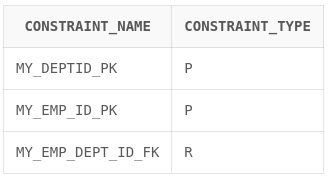
\includegraphics[width=0.5\linewidth]{graphics/p104.png}
\end{figure}

%%%%%%%%% Problem 5 %%%%%%%%%%%

\item Display the object names and types from the \texttt{USER\_OBJECTS} data dictionary view for the EMP
and DEPT tables. Notice that the new tables and a new index were created.

\textbf{Solution: }
\begin{lstlisting}[language=SQL]
SELECT OBJECT_NAME, OBJECT_TYPE
FROM USER_OBJECTS
WHERE OBJECT_NAME IN ('EMP', 'DEPT');
\end{lstlisting}
\textbf{Output: }
\begin{figure}[h]
    \centering
    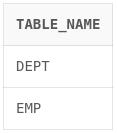
\includegraphics[width=0.3\linewidth]{graphics/p95.png}
\end{figure}

%%%%%%%%% Problem 6 %%%%%%%%%%%
\item Modify the EMP table. Add a COMMISSION column of NUMBER data type, precision 2, scale 2.
Add a constraint to the commission column that ensures that a commission value is greater than
zero.

\textbf{Solution: }
\begin{lstlisting}[language=SQL]
ALTER TABLE emp
ADD commission NUMBER(2, 2);

ALTER TABLE emp
ADD CONSTRAINT chk_commission_positive 
    CHECK (COMMISSION > 0);
\end{lstlisting}

\end{enumerate}



\newpage
\section*{Chapter 8}
\subsection*{Practice 8}
Insert data into the \texttt{MY\_EMPLOYEE} table.
\begin{enumerate}
%%%%%%%Problem 1%%%%%%%%%%%
    \item Run the statement in the \texttt{lab8\_1.sql} script to build the \texttt{MY\_EMPLOYEE} table to be used for the lab.
    
    \textbf{Solution: }
    \begin{lstlisting}[language=SQL]
create table my_employee(
    id number (4) 
        constraint my_employee_id_not_null not null,
    last_name varchar2(25),
    first_name varchar2(25),
    userId varchar2(8),
    salary number (9,2)
);
    \end{lstlisting}
%%%%%%%Problem 2%%%%%%%%%%%
    \item Describe the structure of the \texttt{MY\_EMPLOYEE} table to identify the column names. 
    \begin{figure}[h]
        \centering
        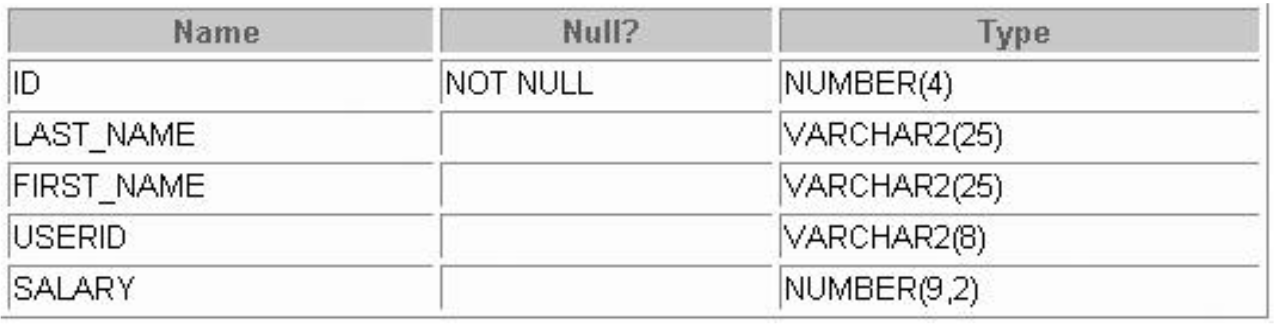
\includegraphics[width=0.7\linewidth]{graphics/82.png}
    \end{figure}
    
    \textbf{Solution: }
    \begin{lstlisting}[language=SQL]
describe my_employee;
    \end{lstlisting}
%%%%%%%Problem 3%%%%%%%%%%%
    \item  Add the first row of data to the \texttt{MY\_EMPLOYEE} table from the following sample data. Do not list the
columns in the INSERT clause.   
    \begin{figure}[h]
        \centering
        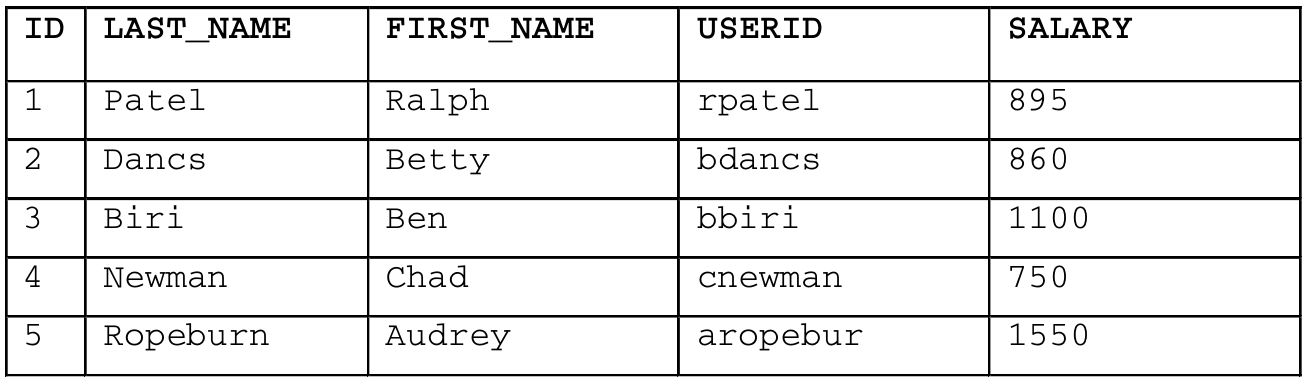
\includegraphics[width=0.7\linewidth]{graphics/83.png}
    \end{figure}

    \textbf{Solution: }
    \begin{lstlisting}[language=SQL]
insert into my_employee
values (1, 'Patel', 'Ralph', 'rpatel', 895);
    \end{lstlisting}
%%%%%%%Problem 4%%%%%%%%%%%
    \item  Populate the \texttt{MY\_EMPLOYEE} table with the second row of sample data from the preceding list. This
time, list the columns explicitly in the INSERT clause.  
    
    \textbf{Solution: }
    \begin{lstlisting}[language=SQL]
insert into my_employee(id,last_name,first_name,userId,salary)
values (2,'Dancs','Betty','bdancs',860);  
    \end{lstlisting}
%%%%%%%Problem 5%%%%%%%%%%%
    \item  Confirm your addition to the table.   
    
    \textbf{Solution: }
    \begin{lstlisting}[language=SQL]
select * 
from my_employee;
    \end{lstlisting}
\begin{figure}[h]
    \centering
    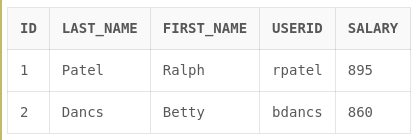
\includegraphics[width=0.7\linewidth]{graphics/p85.png}
\end{figure}
%%%%%%%Problem 6%%%%%%%%%%%
    \item  Write an INSERT statement in a text file named loademp.sql to load rows into the
\texttt{MY\_EMPLOYEE} table. Concatenate the first letter of the first name and the first seven characters of
the last name to produce the user ID.  
    
    \textbf{Solution: }skipped(sql*plus required).
    \begin{lstlisting}[language=SQL]
    \end{lstlisting}
%%%%%%%Problem 7%%%%%%%%%%%
    \item  Populate the table with the next two rows of sample data by running the INSERT statement in the
script that you created. 
    
    \textbf{Solution: }skipped(sql*plus required).
    \begin{lstlisting}[language=SQL]
    \end{lstlisting}
%%%%%%%Problem 8%%%%%%%%%%%
    \item  Confirm your additions to the table.
    \begin{figure}[h]
        \centering
        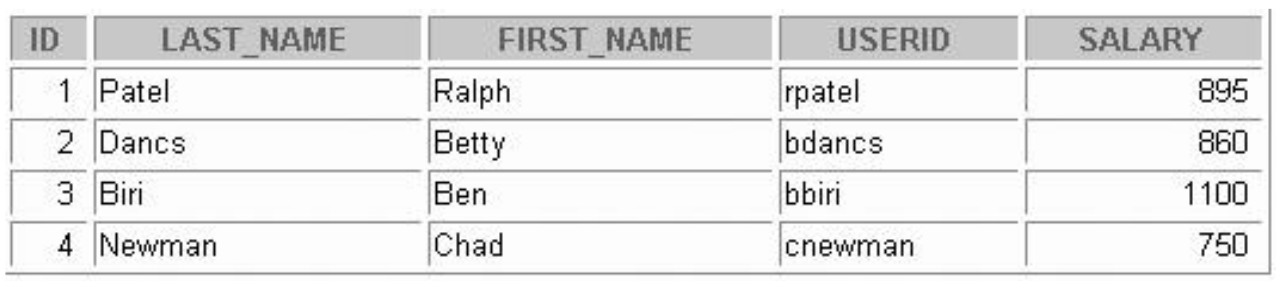
\includegraphics[width=0.9\linewidth]{graphics/88.png}
    \end{figure}
    \textbf{Solution: }
    \begin{lstlisting}[language=SQL]
select *
from my_employee;
    \end{lstlisting}
%%%%%%%Problem 9%%%%%%%%%%%
    \item  Make the data additions permanent.
    
    \textbf{Solution: }
    \begin{lstlisting}[language=SQL]
Commit;
    \end{lstlisting}

Update and delete data in the \texttt{MY\_EMPLOYEE} table.
%%%%%%%Problem 10%%%%%%%%%%%
    \item  Change the last name of employee 3 to Drexler.
    
    \textbf{Solution: }
    \begin{lstlisting}[language=SQL]
-- adding the remaining rows to move forward
insert into my_employee
values (3, 'Biri', 'Ben', 'bbiri', 1100);
insert into my_employee
values (4, 'Newman', 'Chad', 'cnewman', 750);
insert into my_employee
values (5, 'Ropeburn', 'Audrey', 'aropebur', 1550);
    \end{lstlisting}
    \begin{lstlisting}[language=SQL]
update my_employee
set last_name = 'Drexler'
where id = 3;
    \end{lstlisting}
%%%%%%%Problem 11%%%%%%%%%%%
    \item  Change the salary to 1000 for all employees with a salary less than 900.
    
    \textbf{Solution: }
    \begin{lstlisting}[language=SQL]
update my_employee
set salary = 1000
where salary < 900;
    \end{lstlisting}
%%%%%%%Problem 12%%%%%%%%%%%
    \item  Verify your changes to the table.
    
    \textbf{Solution: }
    \begin{lstlisting}[language=SQL]
select id,last_name, salary
from my_employee;
    \end{lstlisting}
    
    \textbf{Output: }
    \begin{figure}[h]
        \centering
        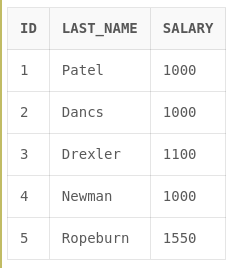
\includegraphics[width=0.4\linewidth]{graphics/p812.png}
    \end{figure}
%%%%%%%Problem 13%%%%%%%%%%%
    \item  Delete Betty Dancs from the \texttt{MY\_EMPLOYEE} table.
    
    \textbf{Solution: }
    \begin{lstlisting}[language=SQL]
delete
from my_employee
where last_name = 'Dancs' and first_name = 'Betty';
    \end{lstlisting} 
%%%%%%%Problem 14%%%%%%%%%%%
    \item  Confirm your changes to the table.
    
    \textbf{Solution: }
    \begin{lstlisting}[language=SQL]
select * 
from my_employee 
where last_name = 'Dancs' and first_name = 'Betty';

--No data found --
    \end{lstlisting} 
%%%%%%%Problem 15%%%%%%%%%%%
    \item  Commit all pending changes.
    
    \textbf{Solution: }
    \begin{lstlisting}[language=SQL]
Commit;
    \end{lstlisting}  
Control data transaction to the \texttt{MY\_EMPLOYEE} table.
%%%%%%%Problem 16%%%%%%%%%%%
    \item Populate the table with the last row of sample data by modifying the statements in the script that you
created in step 6. Run the statements in the script.
    
    \textbf{Solution: }skipped(sql*plus required)
    \begin{lstlisting}[language=SQL]
    \end{lstlisting}  
%%%%%%%Problem 17%%%%%%%%%%%
    \item Confirm your addition to the table.
    
    \textbf{Solution: }skipped
    \begin{lstlisting}[language=SQL]
    \end{lstlisting} 
%%%%%%%Problem 18%%%%%%%%%%%
    \item Mark an intermediate point in the processing of the transaction.
    
    \textbf{Solution: }
    \begin{lstlisting}[language=SQL]
SAVEPOINT before_deletion;
    \end{lstlisting}
%%%%%%%Problem 19%%%%%%%%%%%
    \item Empty the entire table.
    
    \textbf{Solution: }
    \begin{lstlisting}[language=SQL]
delete from my_employee;
    \end{lstlisting}
%%%%%%%Problem 20%%%%%%%%%%%
    \item Confirm that the table is empty.
    
    \textbf{Solution: }
    \begin{lstlisting}[language=SQL]
select *
from my_employee;
    \end{lstlisting}
%%%%%%%Problem 21%%%%%%%%%%%
    \item Discard the most recent DELETE operation without discarding the earlier INSERT operation.
    
    \textbf{Solution: }
    \begin{lstlisting}[language=SQL]
ROLLBACK TO before_deletion;
    \end{lstlisting}
%%%%%%%Problem 22%%%%%%%%%%%
    \item Confirm that the new row is still intact.
    \begin{figure}[h]
        \centering
        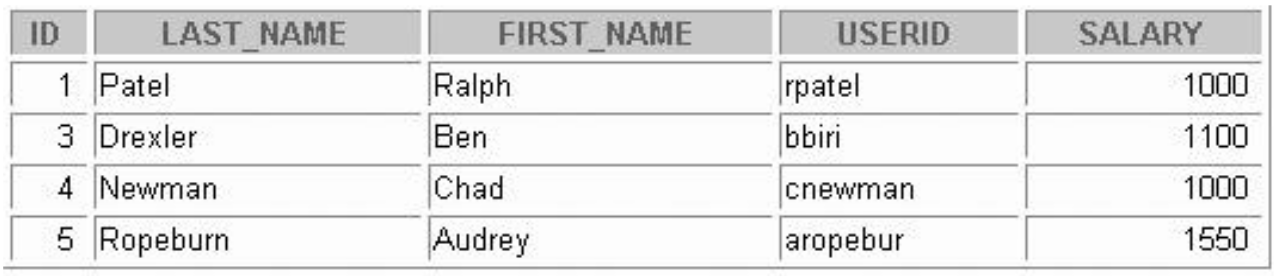
\includegraphics[width=0.9\linewidth]{graphics/822.png}
    \end{figure}

    \textbf{Solution: }
    \begin{lstlisting}[language=SQL]
select *
from my_employee;
    \end{lstlisting}
%%%%%%%Problem 23%%%%%%%%%%%
    \item Make the data addition permanent.
    
    \textbf{Solution: }
    \begin{lstlisting}[language=SQL]
Commit;
    \end{lstlisting}
\end{enumerate}


\end{document}
